\section{PDF space estimators}

We can calculate the same set of estimators in PDF space with minor alteration
to the definitons. Firstly, we are free to choose our own data points which will
be points in x and flavour for the PDFs. For this study we choose the number
of points to be 6. For the singlet and gluon we choose 3 of those points to be
logarithmically spaced between $10^-3<x<0.1$ and 3 to be linearly spaced $0.1<x<0.5$
for the other flavours:  V, V3, V8, T3, and T8 we simply choose the points to be
linearly spaced $0.1<x<0.5$. The covariance matrix which is used in the definition
of bias and variance is estimated from the union of all of the replicas, allowing
for correlations across different flavours. We also calculate $\xi_{1\sigma}$
in the basis which diagonalises this covariance matrix and show that this gives
much better agreement between the expected $\xi_{1\sigma}$ and that measured
directly from the PDFs.

First the ratio of bias/variance for each flavour and total.

\begin{center}
    \begin{tabular}{lr}
        \toprule
        {} &  bias/variance \\
        flavour  &                \\
        \midrule
        $\Sigma$ &           0.58 \\
        gluon    &           0.90 \\
        V        &           0.73 \\
        V3       &           0.77 \\
        V8       &           0.62 \\
        T3       &           0.33 \\
        T8       &           1.18 \\
        Total    &           0.66 \\
        \bottomrule
        \end{tabular}
\end{center}

Now we compare the measured $\xi_{1\sigma}$ with the expected $\xi_{1\sigma}$
calculated from bias/variance.

\begin{center}
    \begin{tabular}{lrr}
        \toprule
        {} &  Measured $\xi_{1\sigma}$ & expected $\xi_{1\sigma}$ from bias/variance \\
        flavour  &                           &                           \\
        \midrule
        $\Sigma$ &                      0.78 &                      0.81 \\
        gluon    &                      0.68 &                      0.71 \\
        V        &                      0.76 &                      0.76 \\
        V3       &                      0.69 &                      0.75 \\
        V8       &                      0.80 &                      0.80 \\
        T3       &                      0.91 &                      0.92 \\
        T8       &                      0.60 &                      0.64 \\
        Total    &                      0.79 &                      0.78 \\
        \bottomrule
        \end{tabular}
\end{center}

For each flavour we can plot $\xi^{i}_{1\sigma}$, the contribution to $\xi_{1\sigma}$
from each of eigenvectors

\begin{figure}
    \centering
    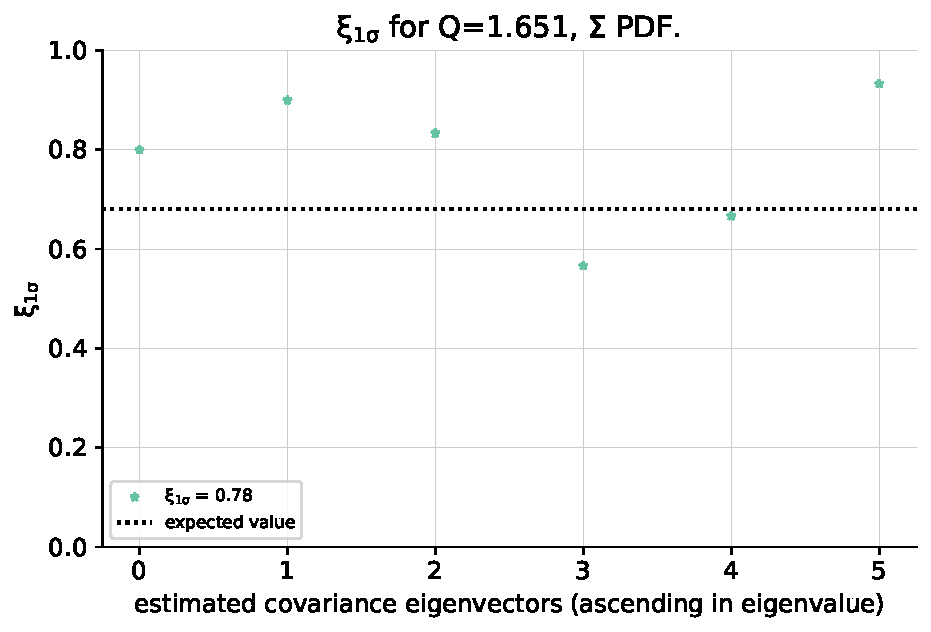
\includegraphics[width=0.6 \textwidth]{diag_sigma.pdf}
    \caption{
        $\xi^{i}_{1\sigma}$ for singlet PDF, in the basis which diagonalises
        the covariance matrix, estimated from the union of all the replicas
    }
    \label{fig:pdfdiagsinglet}
\end{figure}

\begin{figure}
    \centering
    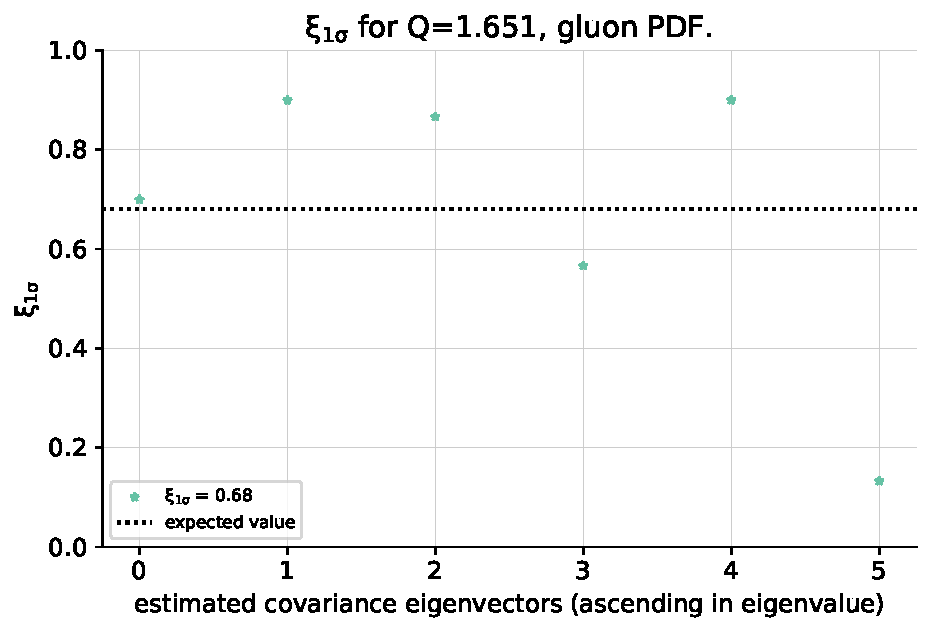
\includegraphics[width=0.6 \textwidth]{diag_gluon.pdf}
    \caption{
        $\xi^{i}_{1\sigma}$ for gluon PDF, in the basis which diagonalises
        the covariance matrix, estimated from the union of all the replicas
    }
    \label{fig:pdfdiaggluon}
\end{figure}

\begin{figure}
    \centering
    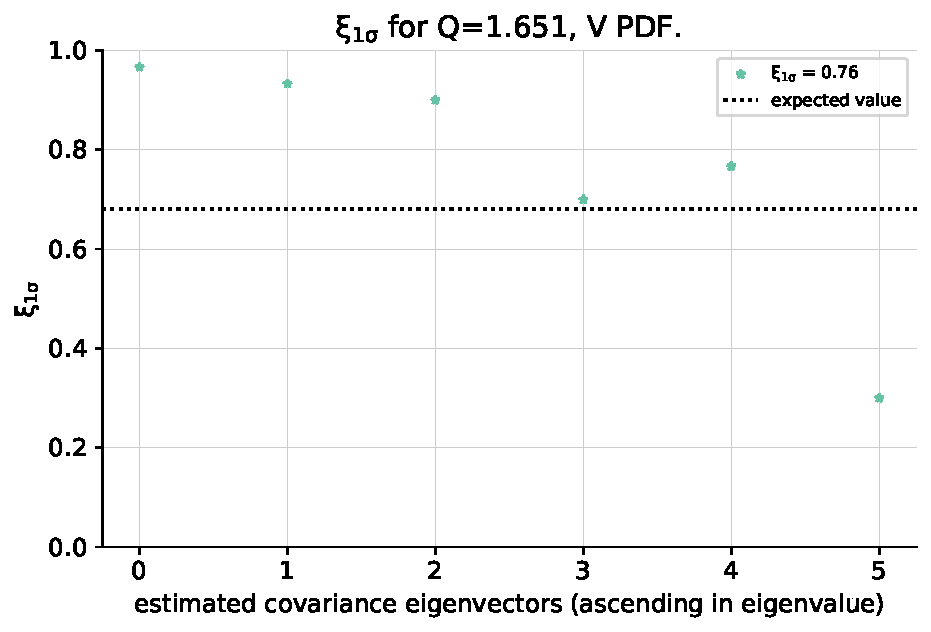
\includegraphics[width=0.6 \textwidth]{diag_v.pdf}
    \caption{
        $\xi^{i}_{1\sigma}$ for V PDF, in the basis which diagonalises
        the covariance matrix, estimated from the union of all the replicas
    }
    \label{fig:pdfdiagv}
\end{figure}

\begin{figure}
    \centering
    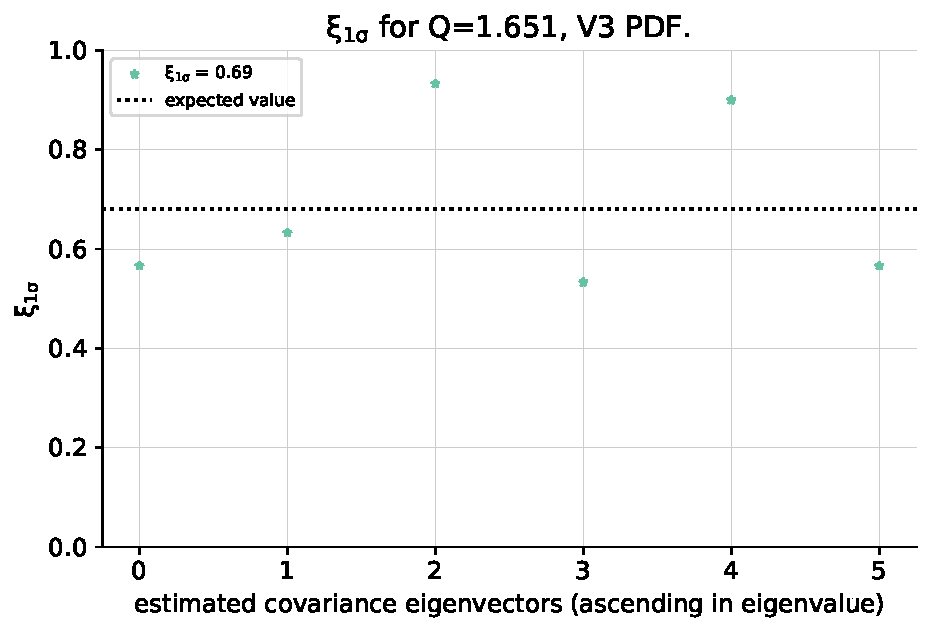
\includegraphics[width=0.6 \textwidth]{diag_v3.pdf}
    \caption{
        $\xi^{i}_{1\sigma}$ for V3 PDF, in the basis which diagonalises
        the covariance matrix, estimated from the union of all the replicas
    }
    \label{fig:pdfdiagv3}
\end{figure}

\begin{figure}
    \centering
    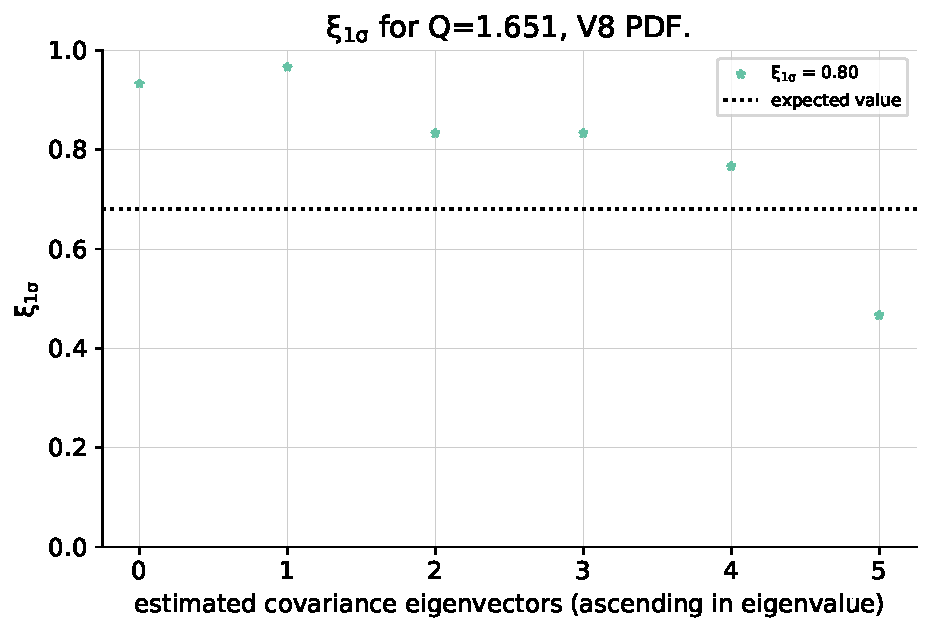
\includegraphics[width=0.6 \textwidth]{diag_v8.pdf}
    \caption{
        $\xi^{i}_{1\sigma}$ for V8 PDF, in the basis which diagonalises
        the covariance matrix, estimated from the union of all the replicas
    }
    \label{fig:pdfdiagv8}
\end{figure}

\begin{figure}
    \centering
    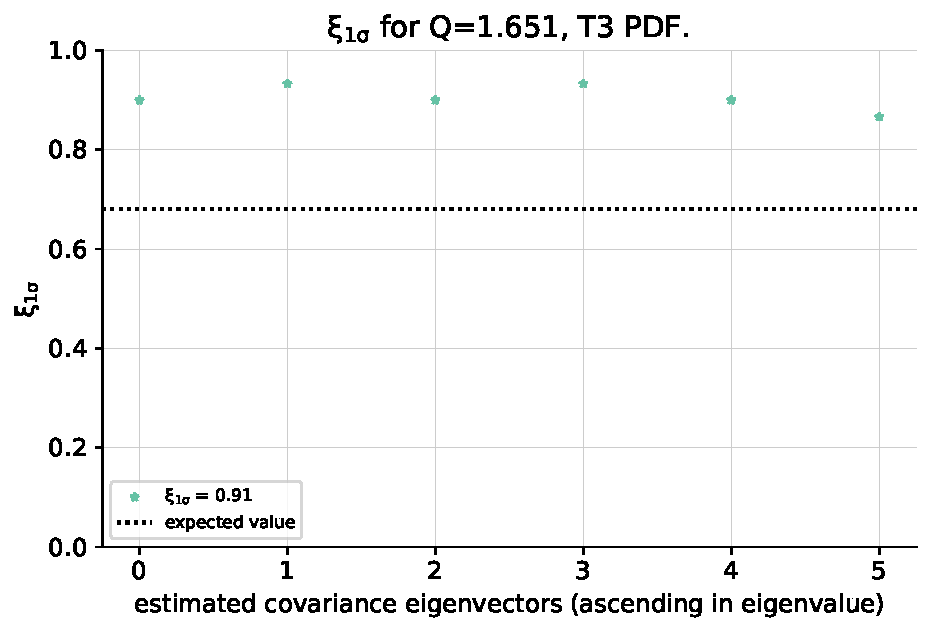
\includegraphics[width=0.6 \textwidth]{diag_t3.pdf}
    \caption{
        $\xi^{i}_{1\sigma}$ for T3 PDF, in the basis which diagonalises
        the covariance matrix, estimated from the union of all the replicas
    }
    \label{fig:pdfdiagt3}
\end{figure}

\begin{figure}
    \centering
    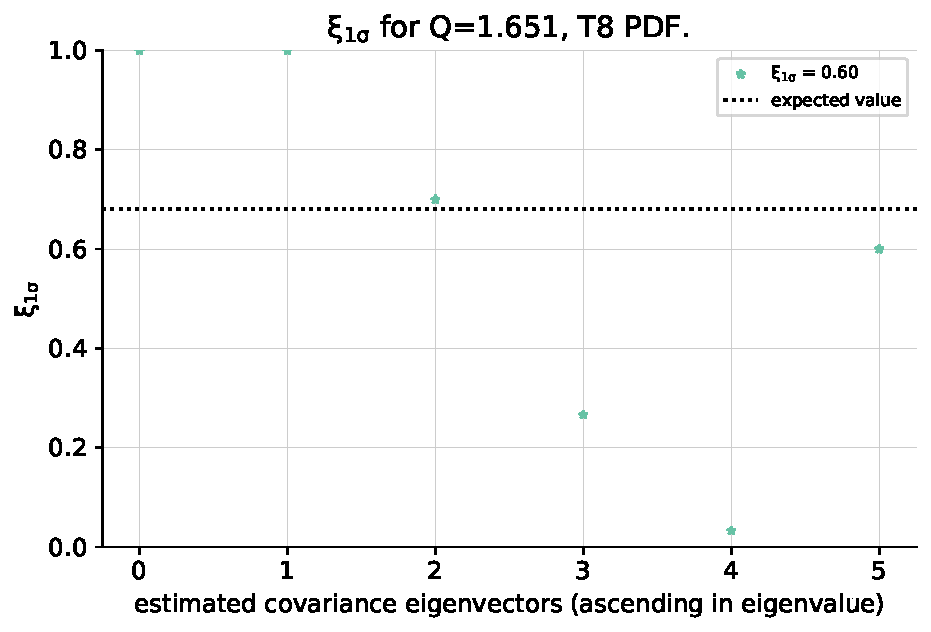
\includegraphics[width=0.6 \textwidth]{diag_t8.pdf}
    \caption{
        $\xi^{i}_{1\sigma}$ for T8 PDF, in the basis which diagonalises
        the covariance matrix, estimated from the union of all the replicas
    }
    \label{fig:pdfdiagt8}
\end{figure}

The PDF results are highly dependent on the number of points chosen in x. Also
the results in the basis which diagonalise the covariance matrix stop us from
seeing how the results depend on x, with the benefit of $\xi_{1\sigma}$ and
the expected results from bias/variance agreeing well. Potentially a far greater
number of fits and replicas are required to get a more reliable result, however
the numbers in the first and second table don't look too bad.
